% Étape 2 : choix de l'entraînement. Sources : notebooks/02_choix_entrainement.ipynb, results/etape2_*.

\section{Choix de l'entraînement}
\label{sec-entrainement}

L'architecture est maintenant fixée ($2\times128$). Nous cherchons comment l'entraîner au mieux, en comparant
les choix vus en cours : l'optimiseur, l'initialisation des poids et la fonction d'activation.

\subsection{Protocole}
\label{sec-entr-protocole}

Nous changeons un seul élément à la fois par rapport à la référence de l'étape 1 : Adam, initialisation de He,
activation ELU (\cref{tab-comparaisons}). Le reste de l'entraînement ne change pas : 200 époques, lots de 32
surfaces, même découpage des données. Comme à l'étape 1, les graines ne changent que l'initialisation des poids
et l'ordre des lots.

\begin{table}[H]
  \centering
  \caption{Les trois comparaisons. La référence est en gras.}
  \label{tab-comparaisons}
  \small
  \begin{tabular}{lll}
    \toprule
    Comparaison & Ce qui varie & Reste fixe \\
    \midrule
    Optimiseurs      & SGD, moment, AdaGrad, RMSProp, \textbf{Adam} & He + ELU \\
    Initialisations  & naïve, Xavier, \textbf{He}                   & Adam + ELU \\
    Activations      & \textbf{ELU}, ReLU, tanh, sigmoïde, GELU, SiLU, linéaire & Adam + He \\
    \bottomrule
  \end{tabular}
\end{table}

Pour que les calculs restent réalisables dans le temps du projet, nous avons allégé cette étape de trois façons.
Chaque configuration est entraînée avec 3 graines au lieu de 5. Le taux d'Adam n'est pas réglé à nouveau : nous
gardons $10^{-3}$, choisi à l'étape 1. Enfin, Leaky ReLU n'est pas testée, afin de limiter le nombre de
configurations. L'étape passe ainsi d'environ 90 à environ 50 entraînements.

La configuration de référence (Adam + He + ELU) est exactement le réseau retenu à l'étape 1 : nous reprenons les
résultats de ses graines 0, 1 et 2, les mêmes graines que pour les autres configurations de cette étape. Sa
moyenne sur ces 3 graines (\num{5.11} $\pm$ \num{0.71}\pb) diffère donc légèrement de celle sur les 5 graines de
l'étape 1 (\num{5.09} $\pm$ \num{0.52}\pb).

\subsection{Réglage du taux de chaque optimiseur}
\label{sec-entr-taux}

Chaque optimiseur a son propre bon taux d'apprentissage. Pour comparer des optimiseurs bien réglés, nous
entraînons chacun avec trois taux, sur une graine (\cref{tab-taux-optim}).

\begin{table}[H]
  \centering
  \caption{Erreur moyenne de validation (pb) selon l'optimiseur et le taux d'apprentissage (une graine).
  Le meilleur taux de chaque optimiseur est en gras.}
  \label{tab-taux-optim}
  \begin{tabular}{lccc}
    \toprule
    Optimiseur & $10^{-4}$ & $10^{-3}$ & $10^{-2}$ \\
    \midrule
    RMSProp & \num{9.7}   & $\mathbf{5{,}6}$ & \num{28.3} \\
    Moment  & \num{70.0}  & \num{32.0}  & $\mathbf{11{,}4}$ \\
    AdaGrad & \num{155.3} & \num{58.7}  & $\mathbf{21{,}3}$ \\
    SGD     & \num{139.0} & \num{70.0}  & $\mathbf{32{,}1}$ \\
    \bottomrule
  \end{tabular}
\end{table}

Le taux compte autant que l'optimiseur. RMSProp passe de \num{5.6} à \num{28.3}\pb\ si le taux est trop grand.
SGD, le moment et AdaGrad, au contraire, sont meilleurs avec le plus grand taux testé : avec un taux plus petit, ils
avancent trop lentement et n'ont pas convergé en 200 époques. Leur meilleur taux étant au bord de la grille, un taux
plus grand pourrait encore les améliorer ; c'est une limite de notre réglage.

\subsection{Résultats}
\label{sec-entr-resultats}

Le \cref{tab-entrainement} donne les erreurs de toutes les configurations et la \cref{fig-comparaisons} leurs
courbes d'apprentissage. Comme à l'étape 1, les erreurs de validation et de test restent très proches (écart
absolu moyen de \num{0.04}\pb, au plus \num{0.18}\pb).

\begin{table}[H]
  \centering
  \caption{Erreur moyenne (pb, moyenne $\pm$ écart-type sur 3 graines) pour chaque comparaison. La référence
  (Adam + He + ELU) est la même dans les trois comparaisons.}
  \label{tab-entrainement}
  \small
  \begin{tabular}{llcc}
    \toprule
    Comparaison & Configuration & Validation & Test \\
    \midrule
    Optimiseurs     & Adam (référence)  & $5{,}11 \pm 0{,}71$ & $5{,}10$ \\
                    & RMSProp           & $5{,}93 \pm 1{,}06$ & $5{,}93$ \\
                    & Moment            & $11{,}4 \pm 0{,}2$  & $11{,}5$ \\
                    & AdaGrad           & $21{,}3 \pm 0{,}2$  & $21{,}4$ \\
                    & SGD               & $32{,}3 \pm 0{,}2$  & $32{,}4$ \\
    \midrule
    Initialisations & Xavier            & $5{,}04 \pm 0{,}39$ & $5{,}03$ \\
                    & He (référence)    & $5{,}11 \pm 0{,}71$ & $5{,}10$ \\
                    & Naïve             & $5{,}31 \pm 0{,}24$ & $5{,}31$ \\
    \midrule
    Activations     & GELU              & $\mathbf{2{,}66 \pm 0{,}09}$ & $\mathbf{2{,}67}$ \\
                    & SiLU              & $2{,}75 \pm 0{,}20$ & $2{,}73$ \\
                    & Sigmoïde          & $4{,}24 \pm 0{,}20$ & $4{,}25$ \\
                    & tanh              & $5{,}05 \pm 0{,}60$ & $5{,}05$ \\
                    & ELU (référence)   & $5{,}11 \pm 0{,}71$ & $5{,}10$ \\
                    & ReLU              & $6{,}16 \pm 0{,}99$ & $6{,}19$ \\
                    & Linéaire (témoin) & $156 \pm 1$         & $155$ \\
    \bottomrule
  \end{tabular}
\end{table}

\begin{figure}[H]
  \centering
  \begin{subfigure}{\textwidth}
    \centering
    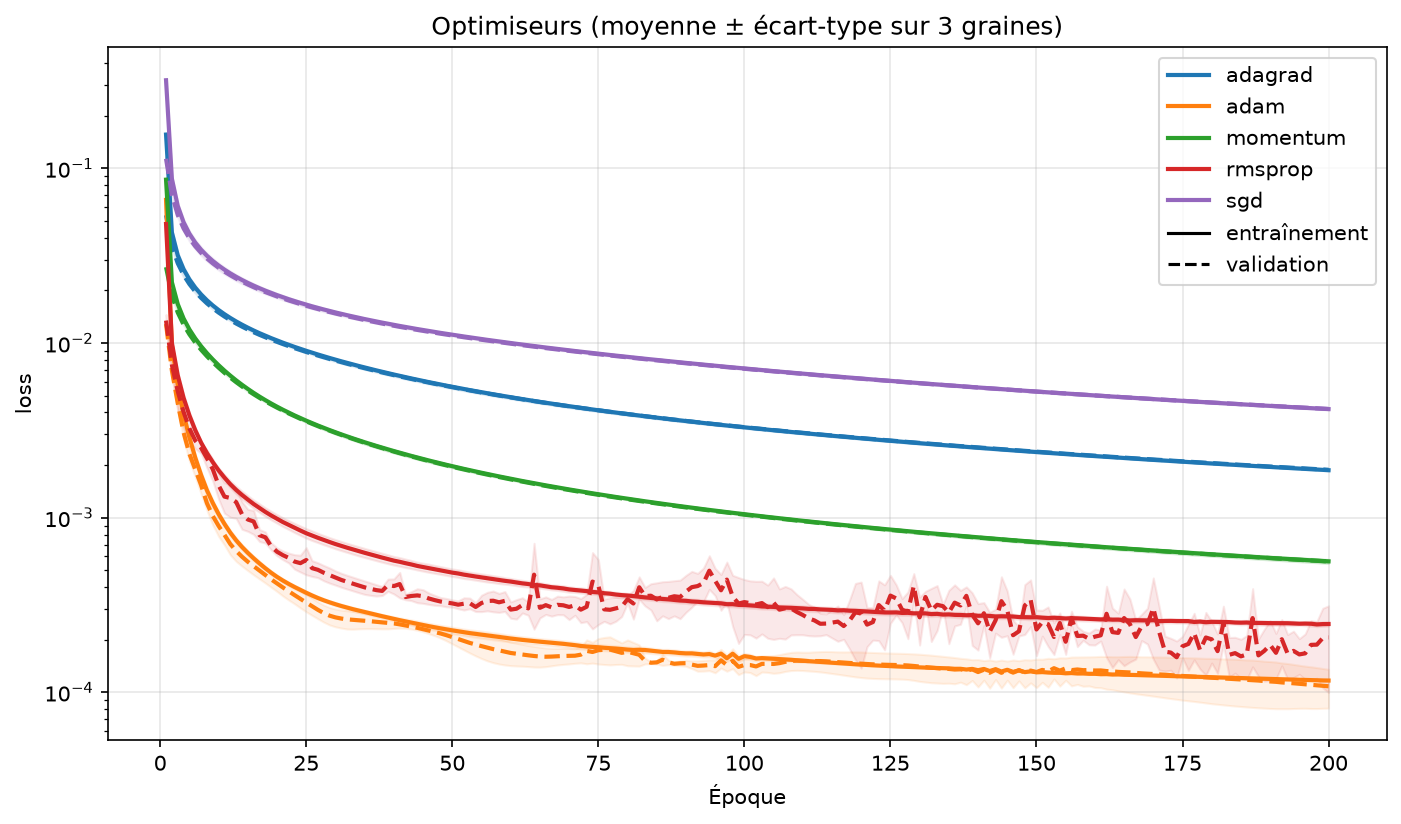
\includegraphics[width=0.62\textwidth]{etape2_serieA}
    \caption{Optimiseurs.}
  \end{subfigure}
  \begin{subfigure}{\textwidth}
    \centering
    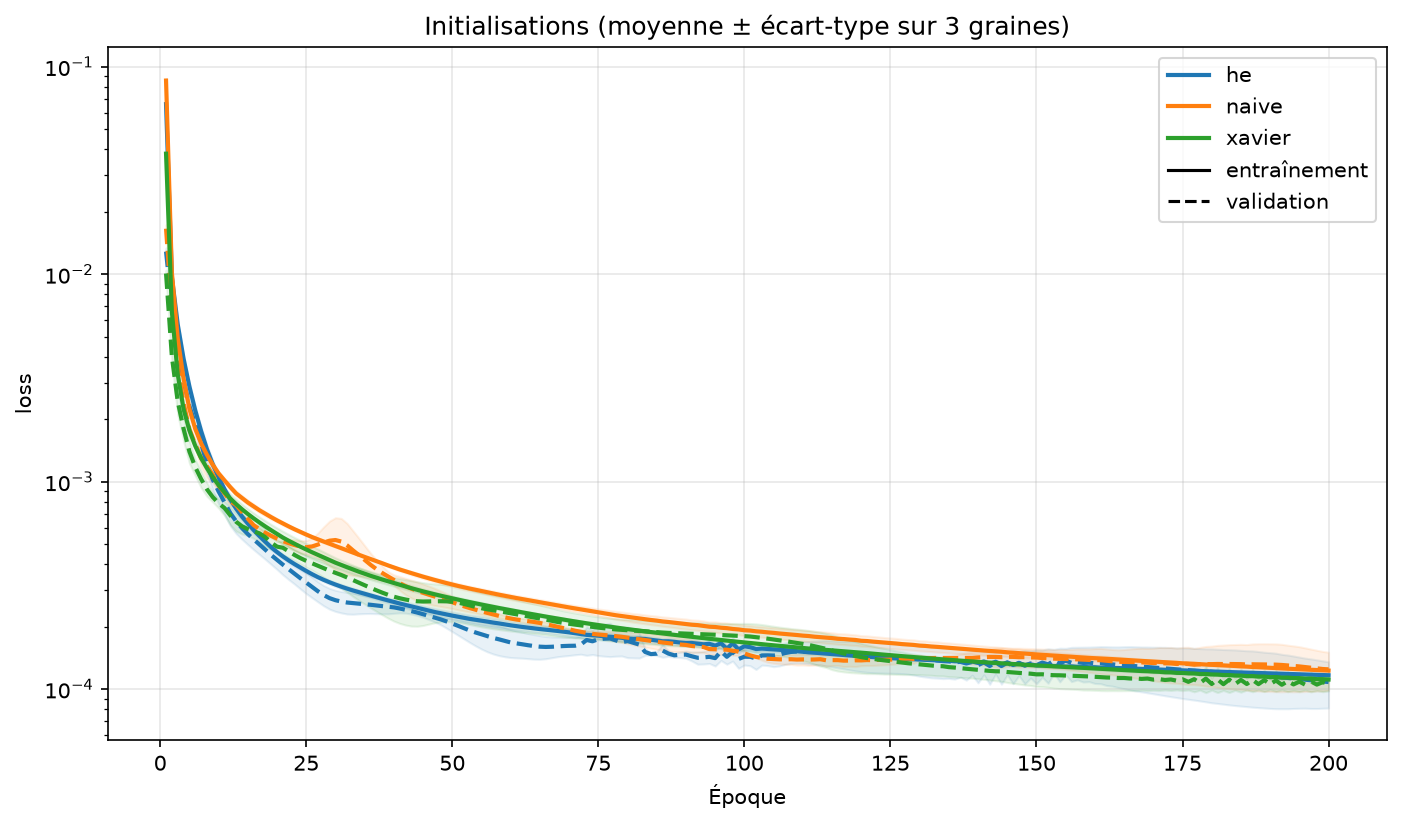
\includegraphics[width=0.62\textwidth]{etape2_serieB}
    \caption{Initialisations.}
  \end{subfigure}
  \begin{subfigure}{\textwidth}
    \centering
    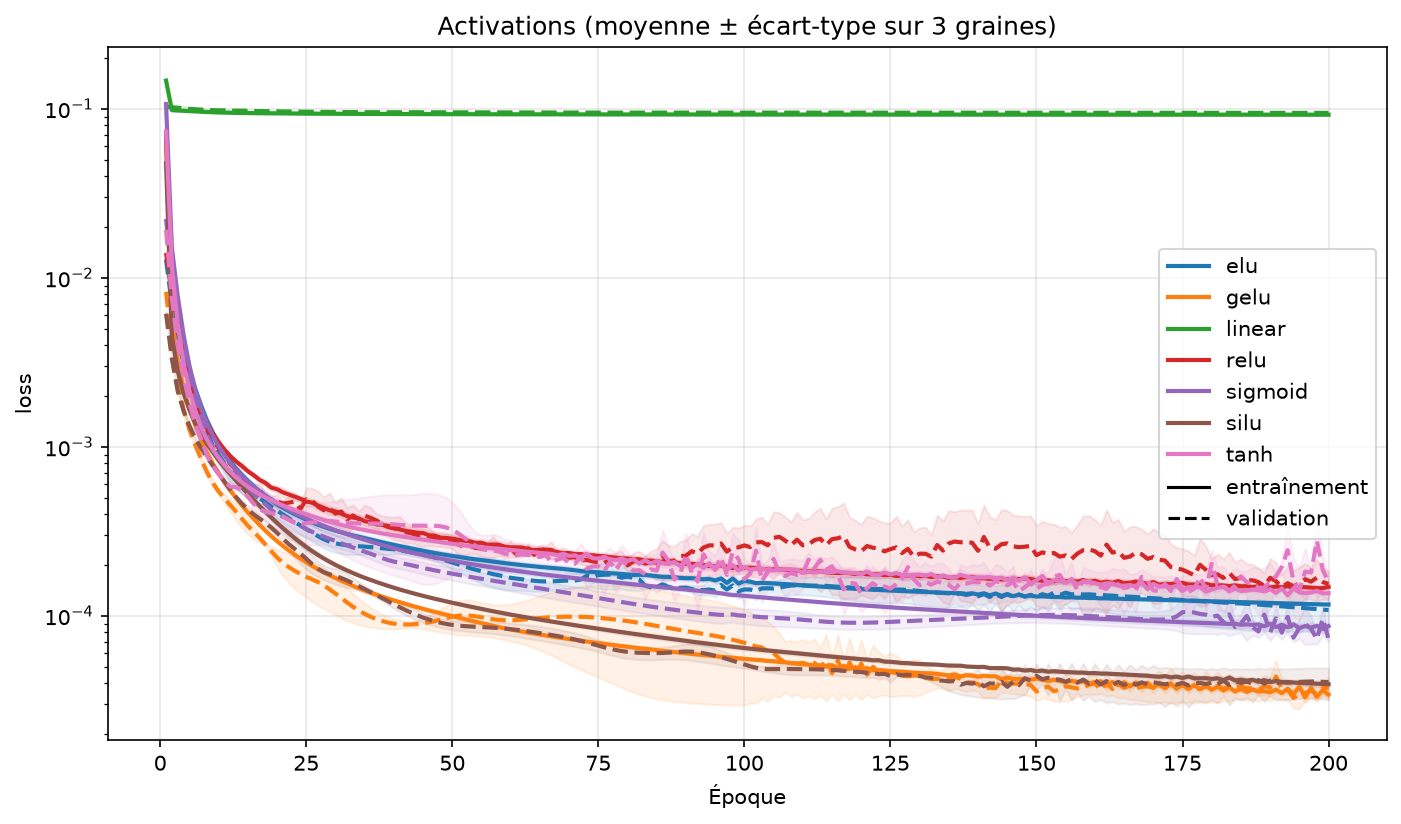
\includegraphics[width=0.62\textwidth]{etape2_serieC}
    \caption{Activations.}
  \end{subfigure}
  \caption{Courbes d'apprentissage : moyenne $\pm$ écart-type sur 3 graines, entraînement en trait plein et
  validation en pointillés.}
  \label{fig-comparaisons}
\end{figure}

C'est l'activation qui fait la plus grande différence dans nos expériences. GELU obtient la meilleure moyenne
observée (\num{2.66}\pb), devant SiLU (\num{2.75}\pb) ; avec 3 graines et ces écarts-types, nous ne pouvons pas
départager ces deux activations. Toutes deux divisent l'erreur par deux par rapport à ELU (\num{5.11}\pb) et font
bien mieux que ReLU (\num{6.16}\pb). Leur caractère lisse pourrait favoriser une approximation régulière de la
surface de volatilité, dont les variations sont elles-mêmes continues ; cette explication reste une interprétation,
que notre expérience ne permet pas d'isoler. Le témoin linéaire, lui, échoue (\num{156}\pb) : sans
non-linéarité, le réseau se réduit à une régression linéaire et ne peut pas représenter la surface.

L'optimiseur compte aussi beaucoup. Adam et RMSProp sont les meilleurs des optimiseurs testés ; le moment, AdaGrad
et SGD restent 2 à 6 fois moins précis, même après réglage de leur taux d'apprentissage. L'initialisation, en revanche, compte peu pour ce réseau de 2 couches :
les trois initialisations sont à moins d'un écart-type les unes des autres.

\subsection{Réseau final}
\label{sec-entr-final}

Nous combinons d'abord le meilleur réglage de chaque comparaison : Adam, initialisation Xavier, activation GELU.
Ces choix ayant été testés un par un, nous vérifions qu'ensemble ils font mieux que la référence. Ce n'est pas le
cas : la combinaison fait \num{2.91} $\pm$ \num{0.14}\pb, moins bien que GELU avec l'initialisation He
(\num{2.66} $\pm$ \num{0.09}\pb). Les meilleurs choix ne s'additionnent donc pas : dans nos expériences, Xavier
est un peu meilleure que He avec ELU, mais la combinaison He + GELU obtient une meilleure moyenne que
Xavier + GELU. Les hyperparamètres interagissent : le meilleur réglage d'un élément dépend des autres.

Le réseau final est le $2\times128$ entraîné avec Adam ($10^{-3}$), l'initialisation de He et l'activation GELU :
\num{2.66}\pb\ sur la validation et \num{2.67}\pb\ sur le test en moyenne sur 3 graines, soit deux fois moins
d'erreur que la référence de l'étape 1, pour le même temps de réponse. Nous gardons la graine la plus précise sur
la validation (\num{2.58}\pb\ sur le test) ; c'est ce réseau qui sert dans la suite.
